\chapter{Introducci'on}
% 
% Existen dos tipos de citas bibliograf'icas: usa \verb|\citep{..}| para
% citas en \emph{par'entesis} y \verb|\citet{..}| para citas
% en el \emph{texto}. Por ejemplo, estudios reciente han mostrado nuevos e
% interesantes modelos que se pueden aplicar para reformular teor'ias
% f'isicas~\citep{NewCam97}. Mientras que, el trabajo de \citet{Rofl06} fue
% considerado muy divertido por una significativa fracci'on de la comunidad
% de investigadores. Tambi'en es posible citar a varios trabajos en una sola
% referencia \citep{Lamport86,Knuth84}.



\section{Propiedades conformacionales de las proteinas}
\begin{itemize}
 \item proteinas globulares, fibrosas y de membrana
 \item folding
 \item estados intermedios de plegamiento
 \item IDPs
 \item misfolding + aggregation + amyloid formation
\end{itemize}


The structure-function paradigm claims that a specific function of a protein is determined by its unique and rigid three-dimensional (3D) structure. 
Thus, following its biosynthesis on the ribosome, a protein must fold to a native, defined 3D structure to be functional. 
The primary origin of this structure-function paradigm is the “lock and key” hypothesis formulated in 1894 by Emil Fischer to explain the astonishing specificity of the enzymatic hydrolysis of glucoside multimers by different types
of similar enzymes. For a long period of time, the validity of “lock and key” model and its associated sequence-structure-function paradigm was unquestioned, especially after the crystal structures of proteins started to be solved by X-ray diffraction

Este paradigma se deriva de los primeros avances en el estudio de estructuras de proteinas. Over the past century evidence steadily accumulated that a well-defined structure is the prerequisite of protein function.



Basic biology and biochemistry textbooks that explain biological phenomena at the molecular level exquisitely rely on this notion, the ‘structure–function paradigm’.

Although deviations from this norm were always apparent, they had been invariably neglected or ignored.
Mas adelante en el tiempo se fue encontrando que, además de las estructuras globulares funcionales mas estudiadas, proteins also populate various other states under native, functional conditions, including disordered and partially ordered conformations, and different aggregated assemblies.
Although it was evident from early studies that both soluble and fibrillar forms of proteins could exist (33 ????) , most attention was focused on the soluble states that were found to possess demonstrable biological function.




En el grafico (*** poner grafico de proteostasis que tiene un estado 'nativo' , un estado 'misfolded' y los demas estados de agregacion, etc) se ve que al sintetizarse, 
la proteina naturalmente tiende a ir adquiriendo una conformacion estructural (conjunto de conformaciones mas restringida).
Lo que se fue desarrollando en los ultimos años es que el estado funcional no pertenece(siempre) a una estructura altamente definida sino que puede pertenecer a un conjunto de conformaciones que van desde
estado plegado hasta estados desestructurados, que pueden confundirse con estados totalmente desordenados. 
% fall onto a structural continuum, from tightly folded single domains, to multidomain proteins that might have flexible or disordered regions, to compact but disordered MOLTEN GLOBULES and, finally, to highly extended, heterogeneous unstructured states 
Thus, not just the ordered state but any of the known polypeptide conformations can be the native state of a protein.

Las sintesis de proteínas en el ribosoma puede verse mejor como el punto de inicio para que cada proteina tome una ruta particular a medida que emerge y se acopla al entorno celular. 
Entre las posibles rutas esta la adquisicion de un continuo de estructuras conformacionales funcionales, la adquisicion de una estructura distinta a la funcional(misfolding), y una variedad de estados de agregacion.

% adquiera un continuo de estructuras conformacionales funcionales a medida q emergen y se acoplan al entorno celular.% adoptando la estructura que la caracteriza .

Es por esto que las propiedades conformacionales de una proteína quedan mejor definidas si se declara el conjunto de multiples estados accesibles por sus estructuras.
% A este continuo de conformaciones que pueden adoptar las proteinas individuales, se agregan distintos tipos de estados agregados, conformados a partir de uniones entre proteinas en distintas conformaciones iniciales(conformaciones desestructuradas, intermedios o plegados).
De acuerdo con esta forma de ver, esta accesibilidad estará dada por la estabilidad termodinámica de cada conformacion accesible y la cinética de interconversión entre estas.
Estos requerimientos pueden indicar por ejemplo q ciertos estados altamente estables como puede ser las fibras amiloides no sean estados naturales comunes debido a los requerimientos cinéticos, a pesar de ser termodinamicamente estables.
% De acuerdo con esta forma de describir las posibles conformaciones de las proteinas, the various fates awaiting a polypeptide chain once it has been synthesized in the cell 
% will depend on the kinetics and thermodynamics of the various equilibria between di¡erent possible states.

Las propiedades cinéticas y termodinámicas están dadas por el contexto celular (pH, iones, concentracion de proteinas, presencia de otras moleculas con las que interactúa, etc) y, obviamente, por los posibles cambios que puede tener una proteina,
ya sean mutaciones o modificaciones postraduccionales.
% Las propiedades estructurales de una proteina, descritas de esta forma, pueden modificarse para una proteina a partir de cambios en el contexto(pH, iones, concentracion de proteinas, presencia de otras moleculas con las que interactúa, etc) 
% y, obviamente, también a partir de mutaciones o modificaciones quimicas sobre ésta. 
Esta forma de ver las propiedades estructurales permite ver los origenes de los cambios conformacionales desde el punto de vista de las propiedades fisicoquimicas de las proteinas.
If the stability or cooperativity of the native state of a protein is reduced, for example by a mutation, the population of non-native states will increase.


Es importante destacar, entonces que, for a given polypeptide chain a chosen fate is not a final one, and a choice may be further modulated by environmental pressure. 
Thus, intrinsically unstructured proteins may be forced to fold or misfold via modification of their environment (addition of natural binding partners, changes in properties of solvent and so on), whereas a destabilizing environment may push a natively
folded protein to the misfolding route. Alternatively, the
presence of chaperones may reverse the misfolding route
and effectively dissolve small aggregates




Durante la última década, uno de los mayores cambios en el campo de las proteínas ha sido el reconocimiento de la ubicuidad e importancia de las proteínas intrínsecamente desordenadas. 
% \cite(INTRINSICALLY UNSTRUCTURED PROTEINS AND THEIR FUNCTIONS)
Las proteinas en solucion fall onto a structural continuum, from tightly folded single domains, to multidomain proteins that might have flexible or disordered regions, to compact but disordered MOLTEN GLOBULES and, finally, to highly extended, heterogeneous unstructured states (FIG. 1) 
% This continuum has been interpreted in terms of a ‘PROTEIN TRINITY’ (ordered, molten globule and RANDOM COIL 20 ) or ‘PROTEIN QUARTET ’ 
As the main criterion of a native protein is its ability to perform a biological function, these partially or completely disordered proteins must be regarded as native entities.

% Si bien decimos aca que las proteinas pueden adquirir estructuras correspondientes un ensamble de estructuras accesibles , es posible hacer una clasificación entre proteinas que adoptan estructuras plegadas(con un estado nativo definido por un pequeño conjunto de estructuras) 
% y proteínas intrínsecamente desestructuradas (que adoptan estructuras correspondientes a un gran ensamble continuo de conformaciones). Luego se tratará las conformaciones agregadas de proteínas como una dimensión conformacional distinta.



% PARA PODER DESCRIBIR DE FORMA SIMPLE LAS PROPIEDADES CONFORMACIONALES SE PUEDE INTENTAR HACER UNA CLASIFICACION DE LAS FORMAS ESTRUCTURALES ADOPTADAS POR LAS PROTEINAS EN SOLUCION. 
% EN FORMA GENERAL SE PUEDEN CLASIFICAR EN:
% 	-CONFORMACION PLEGADA. Este estado nativo puede dividirse ademas en: native (ordered), molten globule, pre-molten globule, and coil-like.
% 	-DISORDERED STRUCTURE (ID): podria considerarse como un conjunto de estados entre los cuales se interconvierte a diferentes velocidades.
% 	-MISFOLDED, AGREGATION,AMYLOID, ETC: generalmente no tienen caracteristicas estructurales definidas, ....




\subsection{Proteinas globulares, fibrosas y de membrana}



% Para intentar clasificar(discretizar)
% the conformational space of globular proteins involves four general conformations(random cloil, pre-molten globules,molten globules, native).

  
% En el caso de proteinas altamente estructuradas, la búsqueda de la estructura nativa no es un proceso trivial, y ha promovido la investigación de estructura de proteínas durante muchos años
% El proceso mediante el cual una proteína adquiere (rápidamente) 
% HACER UNA PEQUEÑA INTRODUCCION AL PROCESO DE PLEGAMIENTO, MUY BREVE
Sin embargo, la idea en esta sección no es hacer un desarrollo del proceso de plegamiento, sino que nos vamos a centrar en las estructuras finales que se pueden encontrar y, cuando sea necesario, en estados intermedios semiestables que sean relevantes.

The sequences of natural proteins have emerged through evolutionary processes such that their unique native states can be found very efficiently even in the complex environment inside a living cell.
Lo que se sabe es que...In order to achieve the native state encoded by the fold, the protein molecule has to find its way to this unique conformation rather than one of the countless alternatives. 
Contemplation of this problem gave rise to the 'Levinthal paradox'. 
In vivo, the beginning of the folding process is the nascent chain as it emerges from the ribosome. 
In vitro, folding begins from a fully formed polypeptide chain that has been unfolded, usually by addition of a chemical denaturant such as urea. 
In both cases the polypeptide chain is highly disordered before folding is initiated. 
In the extreme case, approximated rather well for many proteins in denaturants, the protein is said to be in a `random coil' state, where only local steric interactions constrain the conformations adopted by the molecule.



These intermediates are characterized by substantial secondary structure and little tertiary
structure; a collapsed conformation more compact than the unfolded state; exposed hydrophobic surfaces, 
which lead to binding of hydrophobic dyes
and a propensity to aggregate; 
and a heat capacity similar
to that of the unfolded state. 
The term compact intermediates
encompasses a broad range of conformations
and degrees of
folding and compactness.
compact intermediates have no single, unique conformation, but rather a whole plethora of structures that range from being very
similar to the native state to being substantially expanded and significantly unfolded. 
The properties of compact intermediates from different proteins, and in some cases from the same protein under different conditions, may be significantly different. 
Equilibrium compact intermediates may be good models for transient intermediates formed during folding

Sufficient numbers of different proteins forming stable-equilibrium, partially folded conformations have been observed that we can
make the generalization that all proteins, under the appropriate conditions, will form such species.


The intermediates in the folding process can be classified in
% PONER LOS DISTINTOS ESTADOS INTERMEDIOS





\subsection{Proteinas intrínsecamente desestructuradas}

Varios reviews en \cite{uversky2010understanding,dyson2005intrinsically}.

The suggestion that the native state of many proteins is intrinsically disordered (or, as originally termed, unstructured) is now integral to our general view of protein structure and function.
Como se dijo en la introduccion, a little more than 10 years ago,however, such challenge to the almost dogmatic ‘structure–function paradigm’ was pure heresy due to the overwhelming evidence that structure determines function.
A decade of steady progress turned skepticism around.
Como parte de estos avances, en los ultimos años se han encontrado gran cantidad de proteinas que adoptan estructuras cuyas conformaciones son total o parcialmente desordenadas(segmentos globulares), soportando esta definicion, formalizada a principios de milenio. 
the transition in paradigm was enforced by scattered experimental observations of disorder in a few dozen proteins. 
% una de las dudas que se tenia era si este estado conformacional existia solo in vitro y en realidad in-vivo lo que ocurria era que el crowding generaba el plegamiento
Evidence added to that obtained by other techniques [mostly NMR and circular dichroism (CD)]..... and the evidence seems overwhelming now that structural disorder also exists in vivo and it is truly the native, functional state of these proteins.

En terminos energeticos, for an IDP, the energy landscape is characterized by the lack of a global minimum and by the presence of multiple local minima separated by low energy barriers. 
As a consequence, such a protein exists as a dynamic ensemble of interconverting structures.
Estas secuencias presentan en solución un conjunto heterogéneo de conformaciones fácilmente maleable por cambios en el medio. 
En lugar del análisis estructural clásico basado en dominios globulares, podemos describir estos conjuntos conformacionales en términos de los promedios y desviaciones estándar de la distancia entre los extremos de la secuencia, el radio hidrodinámico, el contenido en estructura secundaria y otros parámetros (20).

Functional complexes of IDPs with their partners are formed via the specific intermolecular interactions that change the energy landscape creating more defined free energy minima.(ESTO LO PODRIA PONER EN LA PARTE DE INDUCED FIT)
A similar mechanism underlies the formation of the non-productive protein complexes (oligomers, amorphous aggregates, amyloid-like fibrils, etc.). Here, interactions of the disordered parts of IDPs or interactions of the denatured proteins result in the appearance of profound free energy minima.

Structurally, IDPs range from completely unstructured polypeptides (native coils, that resemble the highly unfolded states of globular proteins) to extended partially structured forms (native pre-molten globules) or even to compact disordered ensembles that may contain significant secondary structure (native molten globules)
ID proteins have dynamic structures that interconvert on a number of timescales and have been shown to have many similarities to non-native states of “normal” globular proteins, which(como se describio antes) may exist in at least four different conformations: native (ordered), molten globule, pre-molten globule, and coil-like.


Para dejar las cosas un poco mas claras vamos a intentar realizar una clasificacion de las ID proteins en terminos estructurales.
Usando esta analogia(similitud) con los estados intermedios del plegamiento, en \cite{uversky2010understanding} it has been established that ID proteins and regions under physiological conditions in vitro might 
contain collapsed-disorder (i.e., where ID is present in a form of molten globules) and extended-disorder (i.e., regions where ID is present in a form of random coil or pre-molten globule)

\begin{itemize}
 \item[Collapsed disorder: ] The structural properties of the molten globule (which was originally described as universal folding intermediate of globular proteins) are well known and
have been systematized in number of reviews. The protein molecule in this intermediate state has no (or has only a trace of) rigid cooperatively melted tertiary structure. However, it is characterized not only by the well-developed secondary structure, but also by the presence of some topology, i.e., relatively fixed mutual positioning of the secondary structure elements. A considerable increase in the accessibility of a protein molecule to proteases was noted as a specific property of the molten globule.
The transformation into this intermediate state is accompanied by a considerable increase in the affinity of a protein molecule to the hydrophobic fluorescence probes

 \item[Extended disorder: ] A significant number of sequences encodes for the extendedly disordered proteins that are characterized by low sequence complexity. Are these proteins
random coils, or do they possess residual or transient structure? If they have residual or transient structure, how should they be classified? Based on the analysis of the available literature, it has been concluded that such proteins do not possess uniform structural properties, as expected for members of a single thermodynamic entity.
In fact, they may be divided into two structurally different groups, intrinsic coils and intrinsic pre-molten globules, tal como se realiza en \cite{uversky2002natively}: 
 Proteins from the first group have hydrodynamic dimensions typical of considerably unfolded polypeptide chain in poor solvent (see below and fig. 1), and do not possess any (or almost any) ordered secondary structure. 
Proteins from the second group are more compact (see below and fig. 1), and exhibit some amount of residual secondary structure. However, they are still less dense than native globular or molten globule proteins
\end{itemize}



The unfolded protein is essentially never a true random coil. In fact, the existence of significant residual structure in the unfolded globular protein has been described even under the most
severe denaturing conditions, such as high concentrations of strong denaturants [144-147]. Thus, coil-like ID proteins are not completely random, but are characterized by the presence
of some residual (and highly flexible) structure. This fact is very important for the functioning of these proteins.
Protein random coils differ from true random coils in important respects, such as a non-random population of internal bond angles along the chain.

Coincidiendo con esta idea que la proteina no plegada nunca es una true random-coil, the persistence of native-like contacts in the denatured (disordered) state has been shown in NMR experiements and in high temperature molecular dynamics simulation. The existence of preferred limited proteolysis cutting sites also indicates that the native conformation prevails

These and many other studies made the term unstructured obsolete. 
The distinguishing and unifying feature of these proteins,if any, is their inability to fold into a unique and stable tertiary structure.
They display a vast array of function-related structural organization, therefore, the field has settled on the term ‘disordered’. 
This term applies to both short and long regions that are part of a larger folded protein (loops and linkers) and proteins that entirely lack a folded structure. 
This latter category is sometimes also termed (natively) unfolded. 



%  INDUCED FIT:

Many intrinsically disordered proteins undergo transitions to more ordered states or fold into stable secondary or tertiary structures on binding to their targets — that is, they undergo coupled folding and binding processes.

IDPs fold as a whole while interacting with their partners, if the free energy of complex is lower than the free energies of IDP and its partner before their interaction.
More often, however, only a part of an IDP, a specific recognition element, which is a relatively short amphipathic linear motif contained within long disordered sequence, is involved in the coupled folding and binding events
Induced fit interactions can also occur between structural domains and relatively large natively unstructured regions of other proteins. 
The natively unstructured region is then induced to form a stable structure, but only in the presence of the interacting structural domain.

An often-raised issue with respect to IDP binding is whether folding occurs before or after binding (termed conformational selection and induced folding, respectively).
Detailed studies suggest that folding can occur both before and after binding in distinct cases


There are two major models describing the coupled folding and binding process in proteins, the conformational selection model and the simultaneous binding and folding model, also known as the induced folding model.







Ten years ago, only predictor of natural disordered regions (PONDR) was available [14]; today, one can use any of about 50 predictors, which are based on several different principles \cite{he2009predicting}.
Como parte de estos ultimos años de investigacion se encontro una gran cantidad de funcionalidades y mecanismos asociados a proteins IDP(ver seccion funciones).
Se desarrollaron tambien bases de datos específicas (ver disprot, y IDEAL: Intrinsically Disordered proteins with Extensive Annotations and Literature. ) y aplicaciones bioinformáticas capaces de identificar el desorden intrínseco (19).

% The identification of many IDPs  enabled the development of sophisticated bioinformatic algorithms for predicting disorder from sequence, which further advanced the field.
The availability of such predictors further advanced the field.
Based on predictions, we know that structural disorder is abundant in all species, and due to its strong correlation with regulatory and signaling functions, its level is significantly higher in eukaryotes than in prokaryotes
Although it has become almost commonplace in the field that structural disorder increases with the complexity of the organism, the highest levels are not witnessed in the most complex metazoan eukaryotes (e.g., in humans), but in single-celled eukar-
yotes that lead a host-changing lifestyle

% TERMINOLOGIA
En un principio se comenzo a definir a este tipo de secuencias como desestructuradas, indicando que prescindian completamente de estructura, aun sabiendo que they have potentially function-related
short- and long-range structural organization, which eventually called upon a change in terminology.
At that time, high-resolution data were rather limited, thus the concept was mostly phrased from the global structural level, which suggested that IDPs fall into coil-like, pre-molten globuletype and molten-globule types
% aca deberia ir algo sobre estudios estructurales que se han hecho
These and many other studies made the term unstructured obsolete. 
% IMPORTANTE
The distinguishing and unifying feature of these proteins – if any – is their inability to fold into a unique and stable tertiary structure
The terms intrinsically unstructured and natively unfolded may be also be suitable for extended random coils and even those that are collapsed, but these terms don't seem to appropriately describe proteins that form transient or
stable secondary structure. The term disorder suffers because of its negative connotation and its possible confusion with a pathological state, yet, on the other hand, disorder can be used for proteins like the molten globule that form substantial secondary structure but that
nevertheless are highly dynamic and non-uniform. For this last reason, herein we will call these proteins “intrinsically disordered” (ID).
By “intrinsic disorder” we mean that the protein exists as a structural ensemble, either at the secondary or at the tertiary level.

% DISORDER vs FLEXIBILITY:
Disorder and flexibility are often used synonymously, but the two terms are quite distinct\cite{radivojac2004protein}. With regard to an ordered protein, flexibility refers to the magnitudes of the excursions of the atoms from their equilibrium positions.
For a disordered region, variation in flexibility refers to differences in the speed of interconversion among the various members of the structural ensemble. 
A variety of methods have been used to investigate the flexibilities of disordered regions and proteins, including NMR.

Control of structural flexibility is essential for the proper functioning of a large number of proteins and multiprotein complexes. 
At the residue level, such flexibility occurs due to local relaxation of peptide bond angles whose cumulative effect may result in large changes in the secondary, tertiary or quaternary structures of protein molecules. 
Such flexibility, and its absence, most often depends on the nature of interdomain linkages formed by oligopeptides.

Analyses of structures(por ej. mediante X.ray diffraction) have shown that protein motion may occur due to conformational changes in individual residues or at the secondary, tertiary, or quaternary structural levels. Lactate dehydrogenase, triose-phosphate isomerase, as well as hemoglobin and related proteins are some of the earliest examples of proteins that showed conformational changes with important functional implications.




% PROPIEDADES ESTRUCTURALES
A combination of experimental and theoretical studies has clarified how given sequences define specific free energy surfaces that enable folding.
A diferencia de estas superficies energeticas, caracteristicas de las estructuras con plegamiento definido, in some cases the native state of a given peptide or protein may not be structured in a globular form but disordered.
% ESTA LINEA PODRIA IR EN LA PARTE DE HOMEOSTASIS DE PROTEINAS
Regardless of its nature, however, the functional native state is likely to only reflect a local free energy minimum at physiological concentrations, as self-association into aggregated protein spe-
cies may in many cases lower the global free energy 41,42(BOX 1) . Indeed, the maintenance of protein solubility has emerged as a central aspect of the more general topic of protein homeostasis 3,43,44 .

Pero acá estamos hablando de un numero considerable de proteinas cuya secuencia encodes for the intrinsically unstructured proteins without specific structure.
These raise several compelling biophysical questions related to the structural characteristics of natively unfolded proteins. How unfolded are these proteins? Are they random coils, or do
they possess residual structure? If they have residual structure, how should they be classified?
Based on the analysis of the available literature, it has been concluded that intrinsically unstructured proteins do not possess uniform structural properties, as expected for members of a single thermodynamic entity.


In general, proteins with intrinsically disordered sequences cannot bury sufficient hydrophobic core to fold spontaneously into the highly organized 3D structures that characterize the proteins that are represented in the Protein Data Bank (see the online links
box). In some cases, compact but disordered molten-globule-like states can be formed, or local regions of the sequence can have a propensity to adopt isolated and fluctuating elements of secondary structure (which is equivalent to the ‘pre-molten globule’ proposed by Uversky 2 ). 

Structural disorder can now be studied in great detail by several dozen experimental techniques [21], and the most spectacular advance has been achieved through the application of multidimensional NMR. This approach is often
complemented by other structural techniques, such as small-angle X-ray scattering (SAXS), which is combined with advanced computational data integration based upon molecular dynamics (MD) simulations (Figure 1). These new
approaches [22] enabled the characterization of the full structural ensemble of several dozen IDPs

It is probable that proteins rarely, if ever, behave as true random coils, especially in non-denaturing media: even in their most highly unfolded states, proteins show a propensity to form local elements of secondary structure or hydrophobic clusters
Accumulated data nonambiguously show that they most likely represent the polymer coils below a critical point, even under harsh denaturing conditions.




En base a estas propiedades estructurales y el induced fit, en el review \cite{dunker2001intrinsically} se plantea una clasificacion del desorden en dos categorias: intermittent and constant.
The former describes protein molecular recognition domains and other regions that undergo order/disorder transitions to carry out binding or other functions. The latter describes regions such as
roteinaceous detergents, flexible linkers, entropic springs, entropic clocks and entropic bristles that remain disordered while carrying out function.

Two unexpected and important concepts have also emerged in the binding-folding paradigm. One is the intriguing observation that two IDPs/IDRs can bind each other in a process of mutual (synergistic) folding [47].
The other, even more confounding finding, is that recognition can proceed even in the lack of folding in the bound state. 
The many examples of such ‘fuzzy’ interactions demand the extension of the concept of structural disorder to the bound state.




% COMPOSICION

the absence of regular structure in these proteins has been explained by the specific features of their amino acid sequences including the presence of numerous uncompensated charged groups (often negative); 
 i.e., a high net charge at neutral pH, arising from the extreme pI values in such proteins , and a low content of hydrophobic amino acid residues.
Several ID proteins have been discovered due their unusual amino acid sequence compositions

It has been concluded that the combination of low mean hydrophobicity and relatively high net charge represents an important prerequisite for the absence of compact structure in proteins under physiological conditions. This observation was used to develop a charge-hydropathy (CH) plot method of analysis that distinguishes ordered and disordered proteins based only on their net charges and hydropathies.
From the physical viewpoint, such a combination of low hydrophobicity with high net charge as a prerequisite for intrinsic unfoldedness makes perfect sense: high net charge leads to charge-
charge repulsion, and low hydrophobicity means less driving force for protein compaction. In other words, these features are characteristic for ID proteins with the coil-like (or close to coil-
like) structures.
The disordered proteins are significantly depleted in bulky hydrophobic (Ile, Leu, and Val) and aromatic amino acid residues (Trp, Tyr, and Phe), which would normally form the hydrophobic core of a folded globular protein, and also possess low content of Cys and Asn residues.
The depletion of ID protein in Cys is also crucial as this amino acid residue is known to have a significant contribution to the protein conformation stability via the disulfide bond formation or being involved in coordination of different prosthetic groups.
On the other hand, ID proteins were shown to be substantially enriched in polar, disorder-promoting, amino acids: Ala, Arg, Gly, Gln, Ser, Glu, and Lys and also in the hydrophobic, but structure braking Pro.

The fact that natively unfolded proteins, with their depleted hydrophobicity, are noncompact under physiological conditions indicates that ‘salted water’ (typical ‘physiological’ buffer contains 100–150 mM NaCl) does not represent for them a poor solvent.
In other words, these
conditions do not force polymer segments to interact
specifically with each other and, thus, do not force them
to be effectively excluded from the solvent. On the other
hand, it has already been noted that even high concentra-
tions of strong denaturants do not represent a good sol-
vent for a polypeptide chain encoding for a typical glob-
ular protein, and a globular protein was assumed to never
be a random coil.

In addition to amino-acid composition, the disordered segments have also been compared with the ordered ones by various attributes such as hydropathy, net charge, flexibility index, helix
propensities, strand propensities, and compositions for groups of amino acids such as W + Y + F (aromaticity).










Todas estas propiedades hacen que parezca razonable que este tipo de proteínas este altamente regulada dentro de la célula \cite{gsponer2008tight}.



Cada tipo de macromolécula está compuesta por una clase distinta de monómeros. En el caso

\subsection{Misfolding \& Aggregation}

% The sequences of proteins have evolved in such a way that their unique native states can be found very efficiently even in the complex environment inside a living cell. 

contrary to the process of productive protein folding, leading to the appearance of rigid conformation with specific function, the end products of misfolding may have a different appearance. 
The morphology of these end products depends on the particular experimental conditions, and misfolded product may appear as soluble oligomers, amorphous aggregates or amyloid-like fibrils. 
Any of these three species could be cytotoxic, thus giving rise to the development of pathological conditions. 
The reason for such a morphological difference is potentially connected with the diversity of the partially folded intermediates favoring protein self-association. 
In fact, multiple environmental factors, such as point mutations, decrease in pH, increase in temperature, the presence of small organic molecules or metal ions, and other charged molecules, might induce structural rearrangements within a protein molecule, shifting equilirium toward the partially folded conformation(s). As different factors may stabilize slightly different partially folded intermediates, the formation of morphologically
different aggregates is expected.


Como se dijo en las secciones cuando se habló sobre el proceso de plegamiento, las secuencias de proteinas con estructuras plegadas have evolved in such a way that their unique native states 
can be found very efficiently even in the complex environment inside a living cell.


Sin embargo, as the size and complexity of proteins increase, therefore, the folding process becomes more complex. 
Intermediates with only partially formed structures can be populated and have significant lifetimes. 
Under some conditions, then, proteins fail to fold properly or to remain correctly folded; this misfolding can lead to the development of different pathological conditions.
In addition, events that may be termed 'misfolding' may take place during the search for the stable native-like contacts between residues. 
That such complexities are seen even in the benign environment of a dilute solution of a pure protein suggests that they are even more likely to occur in the crowded environment of the cell.

Protein misfolding is a wide-spread phenomenon. Any protein with changes in native structure which affect its normal function is misfolded. 
The terms 'misfolded' and 'aggregated' are not equivalent. Como se verá en las proximas secciones, la habilidad de una proteina formar agregados desestructurados o fibras depende de muchos factores, including protein sequence and environment.
De otra forma, las proteinas que adquieran conformaciones no estructuradas o que se encuentren en estados de plegamiento intermedios semi-estables tendrían una gran tendencia a la agregación, sin embargo esto no es así. 
De hecho, sólo una pequeña fraccion de tales conformaciones tiene tendencia a formar agregados


Undoubtedly,molecular chaperones are able to mitigate some of the consequences of this complex behaviour and provide some protection for the incompletely folded chain. 
But the idea that proteins can misfold, or fold to intermediates that may undergo undesirable reactions such as aggregation, provides insight into potential problems that can arise during folding even in the best designed environments.
Folding and unfolding are also now known to be coupled to many of the key events in the functioning of a biological system, including translocation of proteins across membranes, protein trafficking, 
secretion of extracellular proteins, and the control and regulation of the cell cycle (Radford  Dobson 1999).
Thus, the failure of proteins to fold or to remain folded under physiological conditions is likely to cause malfunctions and hence disease






% **************** AGGREGATION

Although most common forms of proteins are
soluble, some functional states are insoluble,
for example the fibrillar assemblies that form the cellular
cytoskeleton. Proteins are also, however,
vulnerable to forming a wide variety of non-functional
aggregated species. 
Indeed, proteins exhibit generic polymeric and colloidal patterns of behaviour.
Aggregated forms of proteins can be generally amorphous on an ultrastructural level. Of particular fascination, however, because of their
remarkable structures and properties, are highly ordered
self-associated species of peptides and proteins, notably
amyloid fibrils and closely related prion-like states.


Proteins might aggregate into ordered(fibrillar amyloids) or amorphous aggregates structures, utilizing relatively short sequence stretches, usually organized in b-sheet-like assemblies. 
These differences in structure also reflect biological differences; amyloid and amorphous beta-sheet aggregates have different chaperone affinities, accumulate in different cellular locations and are degraded by different mechanisms.

La mayoria de las proteínas forma agregados desordenados, caracterizados por la falta de una estructura tridimensional regular(amorfos).
En condiciones fisiologicas, sin embargo, varias proteinas pueden agregarse formando estructuras altamente ordenadas conocidas como fibras amiloides.
Si bien no se van a dar detalles puntuales de la estructura, se sabe que estas diferencias que se ven en la estructura macromolecular son el reflejo de diferencias en las interacciones y estructura a nivel atómico.


De forma gráfica, los equilibrios de agregacion pueden verse en la figura \ref{aggregationDiagram}

\begin{figure}[h!,centered]
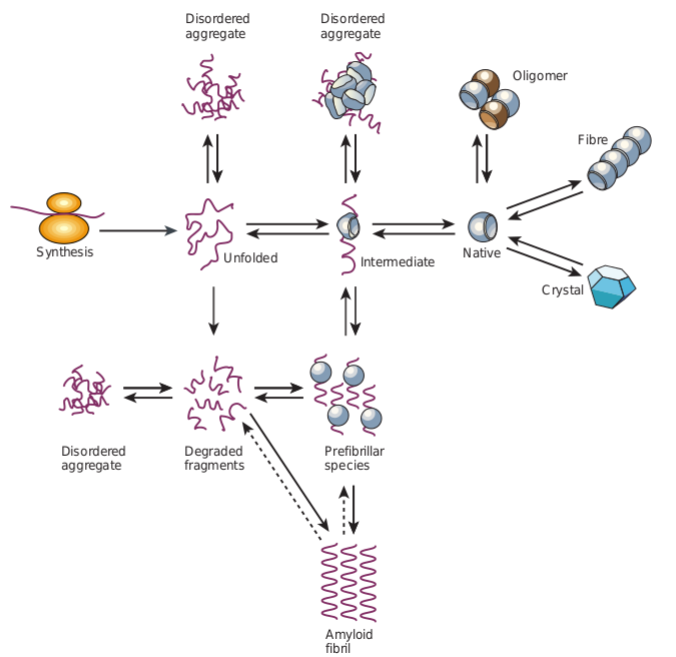
\includegraphics[width=\textwidth]{img/aggregationDiagram.png} 
\caption{Equilibrio de los estados de agregación} \label{aggregationDiagram}
\end{figure}



De la figura puede verse también, que pueden ocurrir distintos procesos de agregación, que resultan en disintas estructuras agregadas, a partir de distintas estructuras adoptadas por las proteinas.



% FIBRAS AMILOIDES: CARACTERISTICAS ESTRUCTURALES Y PROPIEDADES BASICAS
All amyloid fibrils share the same cross-beta archi-
tecture and several functional proteins found in bacte-
ria, fungi, insects and humans have also been found to
adopt the same architecture under physiological condi-
tions, as part of their functional role despite the diversity of origin of their
constituent proteins.













The critical step in the aggregation process is the unfolding of the native structure. 
En la mayoria de las proteinas, excepto las mas pequeñas, el 'unfolding' que ocurre en condiciones fisiologicas no lleva a una estructura totalmente desplegada sino que la proteina adquiere una estructura semi-estable parcialmente collapsada,
donde las interacciones no son las mismas que en el estado nativo estructurado, estas son caracteristicas propias de los intermediarios del plegamiento.

The energy landscape model suggests that some folding intermediates might have structural elements not present in the final folded state.
The appearance of such misfolded intermediates might initiate protein oligomerization or aggregation

La formacion de estos intermediarios es importante porque generalmente son mucho mas solubles que si se formaran conformaciones altamente desplegadas. 
Esta solubilidad permite alcanzar las concentraciones requeridas para la nucleacion propia de la formacion de amyloids(y de agregados en general????)













% ***********************************************************
% ******* PROPIEDADES DE FORMACION DE AMYLOIDS
% ***********************************************************


Since all fibrils independent of the original structure of the given amyloidogenic protein have a common cross-b structure, considerable conformational rearrangements have to occur prior to fibrillation. 
Such changes cannot happen in a native protein, due to its stable and rigid tertiary structure. Thus, protein destabilization favoring partial unfolding and culminating in the formation of a partially unfolded conformation is required. 
Presumably, such a partially unfolded conformation favors reciprocal and specific intermolecular interactions, including electrostatic attraction, hydrogen bonding and hydrophobic contacts, which are necessary for oligomerization and fibrillation
Obviously, this model does take into account a class of natively unfolded proteins, as they are devoid of rigid tertiary structure in their native state.

Data have been reported indicating that the first critical step in protein fibrillogenesis is the partial unfolding of the protein. 
Due to structural fluctuations (conformational breathing) the structure of a globular protein under physiological conditions represents a mixture of tightly folded and multiple partially unfolded conformations, 
with great prevalence of the former. 
Most mutations associated with accelerated fibrillation and protein deposition diseases have been shown to destabilize the native structure, increasing the steady-state concentration of partially folded conformers

Detailed structural analysis of early fibrillation events in several proteins has demonstrated that the amyloidogenic conformation is only slightly folded and shares many structural properties with the premolten globule state.

This picture enables us to speculate on the origins of the amyloid diseases from the point of view of the physico-chemical properties of the protein molecules. If
the stability or cooperativity of the native state of a protein is reduced, for example by a mutation, the population of non-native states will increase.
This rise will increase the probability of aggregation, as the concentration of polypeptide chains with at least partial exposure to the external environment will be greater. Whether or not aggregation does occur will depend on
the concentration of protein molecules, the intrinsic propensity for a given sequence to aggregate when unfolded, and on the rate of the aggregation process. The
fact that formation of ordered amyloid fibrils can be seeded, like the well-studied processes of crystallization
and gelation, means that once the aggregation process is initiated it often proceeds very much more rapidly.
In the absence of seeding there can be long 'lag' phases before aggregation occurs . This lag can be thought of as arising because the growth of a fibril cannot occur until a 'nucleus' of a small number
of aggregated molecules is formed. Such a nucleus can be formed by the local £uctuations in concentration that occur in solution as a result of random molecular motion. When such fluctuations result in a local concentration of
molecules above a critical value, the molecules associate with one other to form a species that is suficiently large to have intrinsic stability, and hence to grow in size by interacting with other molecules in the solution. The act
of seeding provides such nuclei to the solution and hence reduces or abolishes the lag phase

The proposal that amyloid fibrils are a generic structure of polypeptide chains (se desarrolla mas adelante en la parte de amyloids) coincide con esta forma de ver.

% The amyloid conformation reflects an intrinsic conformational propensity of polypeptides as many proteins can be forced into amyloid fibrils by manipulating external conditions. 
Several observations (por ejemplo que ordinary peptides and proteins can convert under appropriate laboratory conditions into aggregates with all the characteristics of the amyloid fibrils),
together with a wide variety of biophysical and computational studies, led to the suggestion that the amyloid structure can in principle be adopted by any polypeptide chain.
The amyloid state of a protein is therefore generic, as it is accessible to many different polypeptide chains, and, unlike the native state, its essential architecture is not encoded by the amino acid sequence,
although the details of its structure and stability can be markedly sequence-dependent, as we discuss below. 
% Despite active research, a detailed understanding of the molecular principles underlying the transformation of soluble proteins into amyloid aggregates is still lacking

% However, amyloid formation is also a sequence-specific process 14,15 .
Even though the ability to form amyloid fibrils seems to be generic, the propensity to do so under given circumstances can vary markedly between different sequences.
Under physiological conditions, most peptide sequences derived from proteins will remain soluble even at high concentrations, whereas most hydrophobic sequences will invariably aggregate as amorphous aggregates.

Similar to globular native states, amyloid structures are closely packed and highly ordered



Amyloidogenic proteins are quite diverse, with little similarity in sequence and native three-dimensional structure.
Additionally, several proteins and peptides not related to amyloidoses have the potential to form amyloid fibrils in vitro, suggesting that this ability for structural rearrangement and aggregation may be inherent to proteins.
Even though the ability to form amyloid fibrils seems to be generic(is a general property of the polypeptide backbone), the propensity to do so under given circumstances can vary markedly between different sequences(depends enormously on amino acid composition.).

This picture enables us to speculate on the origins of
the amyloid diseases from the point of view of the
physico-chemical properties of the protein molecules. If
the stability or cooperativity of the native state of a
protein is reduced, for example by a mutation, the popu-
lation of non-native states will increase.
This rise will increase the probability of aggregation, as the
concentration of polypeptide chains with at least partial
exposure to the external environment will be greater.
Whether or not aggregation does occur will depend on
the concentration of protein molecules, the intrinsic
propensity for a given sequence to aggregate when
unfolded, and on the rate of the aggregation process. The
fact that formation of ordered amyloid fibrils can be
seeded, like the well-studied processes of crystallization
and gelation, means that once the aggregation process is
initiated it often proceeds very much more rapidly.
In the absence of seeding there can be
long 'lag' phases before aggregation occurs .
This lag can be thought of as arising because the growth
of a fibril cannot occur until a 'nucleus' of a small number
of aggregated molecules is formed. Such a nucleus can be
formed by the local fluctuations in concentration that
occur in solution as a result of random molecular motion.
When such fluctuations result in a local concentration of
molecules above a critical value, the molecules associate
with one other to form a species that is suficiently large
to have intrinsic stability, and hence to grow in size by
interacting with other molecules in the solution. The act
of seeding provides such nuclei to the solution and hence
reduces or abolishes the lag phase







% **********************
% AGREGADOS AMORFOS
% **************************

Amorphous beta-sheet aggregation, is less position-dependent(than amyloid aggregation) and can, in principle, be achieved by any sequence that can adopt an extended conformation, is sufficiently hydrophobic and has no unsatisfied hydrogens or electostatic groups. 
Thus beta-sheet aggregation can be relatively easily predicted by methods that evaluate aggregation by evaluating biophysical parameters over a sequence segment, without the need for considering position-dependent values of these parameters.





% AGREGACION DE PROTEINAS IDPs

%Many proteins adopt various other biologically relevant conformational states in addition to their native structure. 
%These partially folded protein species are particularly vulnerable to misfolding and aggregation from which they must be protected in living systems

Intrinsically disordered proteins are not necessarily prone to aggregation, as their sequences have usually evolved to maintain the level
of solubility that is required for their optimal function; for example, through the existence of extensive regions that are highly abundant in charged and polar groups
that disfavour intermolecular association from a thermodynamic point of view. 
Moreover, as is discussed below, kinetic barriers to aggregation are crucial in enabling both globular and disordered proteins to maintain their soluble and functional states





% FUNCTIONAL AMYLOIDS
Amyloids are not only associated with disease-related proteins.
Nature also exploits the structural and mechanical properties
of amyloids to regulate biological functions 13 . For example, in
bacteria amyloids such as curli promote biofilm formation and
host invasion, and chaplins in bacteria and hydrophobins in yeast
act as regulators of surface tension of water. Insects and fish
use chorion amyloid as a component of eggshell, and spiders
use spidroins in spider silk. Humans possess at least one func-
tional amyloid protein: Pmel17 is used as a structural scaffold
in melanin synthesis. The strength and flexibility of amyloids
have attracted attention for their use as biomaterials. However,
it remains to be understood how functional amyloids avoid the
cytotoxic effects observed in disease amyloids. In part, functional
amyloids are regulated by chaperones and proteases. But it is
also becoming evident that sequence composition modulates
critical biophysical parameters determining kinetics of assembly
or mechanical strength.




\subsection{Mecanismos naturales de proteostasis}
En secciones previas(en la introduccion) se dijo que el espacio de conformaciones accesibles por las proteinas dependia de las estabilidades termodinamicas de los estados y la cinetica de interconversión entre estos. 
Estas propiedades, a su vez, dependen del contexto celular en el que se encuentran(ademas de la secuencia de la proteina en si misma), concentraciones de proteinas, localizacion, interacciones, etc.
El balance correcto entre todas estas condiciones está regulado a traves del proceso de proteostasis.
Proteostasis refers to controlling the concentration, conformation, binding interactions (quaternary structure), and location of individual proteins making up the proteome by readapting the innate biology of the cell, 
often through transcriptional and translational changes.
The protein components of eukaryotic cells face acute and chronic challenges to their integrity. Eukaryotic protein homeostasis, or proteostasis, enables healthy cell and organismal development and aging and protects against disease
Los mecanismos dentro del proceso de proteostasis permiten successful organismal development and aging in the face of constant intrinsic and environmental challenges %previniendo el desarrollo de enfernedades.

The healthy state of a cell is characterized by a detailed balance between the different states that proteins can populate. 
Perturbations to such balance, unless they are kept under strict control, can lead to deleterious events and disease.


La proteostasis es influenciada por todos los mecanismos que controlan los aspectis vistos en las secciones previas..... by the chemistry of protein folding/misfolding and by numerous regulated networks of interacting and competing biological pathways 
that influence protein synthesis, folding, trafficking, disaggregation, and degradation.

La celula posee distintos mecanismos para regular estos procesos .....chaperonas para regular el proceso de folding/misfonding (y tambien de aggregation), 
Nature developed very sophisticated protection mechanisms (chaperones, proteasome, etc.) for the effective regulation of the folding process, y por lo tanto prevenir las peligrosas consecuencias de misfolding. 
In other words, in the cell, any given protein is not acting in the isolation, is never alone and is
constantly "watched" by the protective machinery. This machinery is rather robust and can
tolerate significant loads. Obviously, factors that affect these protective mechanisms will
contribute to the probability of disease development


-Cells possess a complex proteostasis network (PN) to ensure protein homeostasis.
-Aggregates permanently engage molecular chaperones and other PN components.
-The PN is challenged by chronic stress in protein-aggregation diseases and aging.
-Overtaxing the PN drives a vicious cycle of disease progression with eventual proteostasis collapse.



Las diferencias estructurales vistas entre los distintos estados de agregación tambien se ven reflejada en diferencias biológicas 
Whereas misfolded and aggregated proteins are found in perinuclear locations and are generally degraded by the 
proteasomal system, amyloids preferentially accumulate in perivacuolar inclusions, where they are degraded by the autophagosome.
% This segregation directly results from a differential recognition by the protein quality control system. 
Esta segregación resulta en un tratamiento distinto por parte de los mecanismos encargados de la proteostasis.
A reduced affinity of amyloids for the protein quality control system is probably also at the root of their higher toxicity 11 as artificial overexpression of chaperones
usually leads to decreased toxicity and removal of amyloids from he cell.
Contrary to amorphous aggregates, amyloid structures can fulfill biological functions, and functional amyloids are found in organisms from prokaryotes to humans \cite{fowler2007functional}.





% PREVENCION DE AGREGACION EN FOLDED PROTEINS
the normal folding process may pass through
partially folded states on the route to the fully native state,
but the aggregation of these species will be minimized by
the presence of molecular chaperones. In addition, if the
protein is able to fold rapidly, any partially folded species
will have a short lifetime, reducing the probability of inter-
molecular interactions occurring. Moreover, once folded,
the native state is generally a highly compact structure
that conceals the polypeptide main chain within its
interior. Such a state is protected from aggregation except
through the interactions of surface side chains (as is the
case, for example, in protein crystals) and is unable to
form the strong intermolecular hydrogen bonds associated
with the polypeptide backbone. Provided that the native
state is maintained under conditions where it remains
folded, aggregation to amyloid fibrils will be resisted by
the kinetic barrier associated with unfolding, even if the
aggregated state is thermodynamically more stable.
Importantly, the cooperative nature of protein structures
means that virtually none of the polypeptide chain in indi-
vidual molecules is locally unfolded, and that virtually no
molecules in an ensemble are globally unfolded, even
though native proteins are only marginally stable relative
to denatured ones under normal physiological conditions


% ACA EXPLICO POR QUE LAS IDPs NO TIENEN TANTA TENDENCIA A FORMAR AGREGADOS
In contrast to the globular proteins, which have to unfold prior to aggregation (Jahn and Radford, 2005), IDPs are always ready for intermolecular interactions. 
An unbound fragment of an IDP possesses a strong ability to interact, and therefore can bind either to natural partners forming native complexes or to similar molecules forming various aggregates. 
This raises the question of why IDPs do not always form aggregates in the norm. One of the potential answers is the fact that inside the cell, the IDPs typically form complexes with natural partners.
Los mecanismos de proteccion (chaperonas, proteasoma, etc) tienen una gran capacidad para mantener la solubilidad de proteinas.
Además, based on the analysis of the IDP amino acid composition, it would be clearly a mistake to assume that an averaged IDP possesses higher propensity towards aggregation than an averaged ordered
protein. In fact, many IDPs contain large number of charged and polar residues. In addition to the hydrophobic interactions, the net charge is one of the major factors determining aggregation behavior of a protein.













\section{Características funcionales}
\begin{itemize}
 \item Breve historia estructura-función
 \item motivos secuenciales
 \item funcionalidad en proteinas IDPs
\end{itemize}


This means that the structure-function paradigm, which emphasizes that ordered 3D structures represent an indispensable prerequisite to effective protein functioning, should be redefined to include intrinsically unstructured proteins [159]. According to this redefined paradigm, native proteins (or their functional regions) can exist in any of the known conformational states, ordered, molten globule, premolten globule and coil. Function can arise from any of these conformations
and transitions between them. Thus, not just the ordered state but any of the known polypeptide conformations can be the native state of a protein.




% FUNCIONALIDAD EN IDPs

% HASTA ACA DEBERIA HABER DEFINIDO TODOS LO QUE RESPECTA A ESTRUCTURA-FUNCION EN DOMINIOS GLOBULARES
En las secciones anteriores se mostro como es la realidad en cuanto a la conformacion de proteinas en su estado nativo, entre las cuales podemos encontar gran variedad de proteinas funcionales que no adoptan una estructura tridimensional definida
y por lo tanto no se ajustan a este paradigma de estructura funcion, aunque si se sabe que cumplen funciones celulares relevantes.
The most important question of the field, therefore, is the physiological function and functional mode of IDPs/IDRs.


IDP functions either directly stem from their disorder (entropic chains) or from molecular recognition, when they undergo induced folding (disorder-to-order transition) upon binding to a partner molecule
The functional role of structural disorder from a biological process view addresses what type of cellular functions benefit most from the lack of a stable structure. This question was addressed in several large bioinformatics studies. 
As a result, IDPs are generally thought to be involved in processes of signaling and regulation, and in depth correlation analysis [52] of 710 Swiss-Prot functional keywords suggested significant positive correlation with 238 functions and negative correlation with 302 functions (Table 2). 
Most of the functions that correlate with the presence of long disordered regions are related to regulation via transcription and translation, whereas functions that correlate with the lack of disorder are dominated by enzymatic catalysis.

Algunas propiedades interesantes de las proteinas IDPs se revelan a partir de estudios a nivel de proteoma y sistema.
As a result of breathtaking advances in comparative evolutionary and experimental structure–function studies, it is now clear that the intrinsic lack of structure and function-related disorder-to-order transitions provide
IDPs with various functional advantages\cite{gunasekaran2003extended,dyson2005intrinsically}, such as: (i) Decoupled specificity and strength of
binding provides for high-specificity-low-affinity interactions; 
(ii) Increased speed of
interaction due to greater capture radius(and it can bind at a relatively larger distance
followed by reeling on to the partner, potentially enhancing
the rate of binding by a ‘fly-casting’ mechanism, according to which the unfolded polypeptide first binds weakly at a relatively large
distance from the actual binding site and then folds as the protein approaches the binding
site)
and the ability to spatially search through
interaction space (ie. in the spatial search by transcription factors
in sequence-specific DNA recognition, termed the ‘monkey-
bar’ binding mechanism);
(iii) Increased interaction (surface) area per residue; (iv) The ability for
one-to-many and many-to-one interactions; (v) Increased capture radius for a specific
binding site in comparison with that of ordered protein with its restricted conformational
freedom, (vi) Fast binding kinetics, etc

Intrinsic plasticity has been proposed to be advantageous because it could enable a single protein to recognize many biological targets while still being specific
Moreover, it has been pointed out that the susceptibility to proteases and, hence,
shortened lifespan of disordered proteins is an added advantage because these proteins play roles in cell-cycle
regulation


Ademas, Disordered proteins often have
large intermolecular interfaces, the size of which is dic-
tated by protein function. For proteins to be stable as
monomers with extensive interfaces, protein size
would need to be 2–3 times larger. This would either
increase cellular crowding or enlarge the size of the cell
by 15 –30\%, owing to the increase in the sequence
length. Smaller sizes of cells, proteins, DNA and RNA
conserve energy. Thus, disordered proteins provide a
simple yet elegant solution to having large intermolecu-
lar interfaces, but with smaller protein, genome and
cell sizes.
The natively disordered state is a simple
and elegant solution adopted by evolution to avoid large
protein, genome and cell sizes.

For many examples, the given disordered regions are not known to bind to any partner, but they still carry out
important functions such as providing flexible linkers be-
tween structured domains or providing flexible tails that
regulate the structured domains

Several of their specific functional modalities, such as adaptability in binding, high functional density, weak but specific binding, and frequent regulation by post-translational modification, have been formally demonstrated. 


Even if the lifetime of the preferred native
conformation is short(como es el caso de las disordered conformations), this conformation still exists. The
binding and shift in the equilibrium takes care of
the function.


% ACA CONECTO CON SLM
The induced folding concept stimulated much research and led to a virtual explosion in the field of short motifs.
As suggested, IDPs/IDRs often function by binding accompanied by induced folding (molecular recognition) [6–8] mediated by SLiMs/ELMs, and in several recent
works it has been shown that the functional and evolutionary agility of IDPs can be ascribed to the inclusion or exclusion of such motifs in RNA maturation; that is, by alternative splicing, alternative promoter usage, and RNA
editing, the alternative isoforms thus generated promote the functional diversification of the proteome
This mechanism can result in a change in diverse functional attributes, such as subcellular localization, protein–protein interaction, phase transitions and even opposing (dominant negative) function, as also demonstrated by
studying tissue-specific forms of alternative splicing. These protein isoforms tend to occupy central positions in interaction networks and their pattern of interaction partners tend to significantly differ [63]; that is, structural disorder
and encoded motifs have a strong potential to define and redefine wiring of cellular signaling pathways.





% **************************************************
% LINEAR MOTIFS VISTOS COMO UNIDADES MODULARES QUE COMPONEN A LAS PROTEINAS
% *****************************************************
Como se puede ver en el trabajo \cite{neduva2005linear}.....
Proteins are usually modular, containing discrete regions each of which performs a different sub-function. 
The most widely known modular element is the protein domain. These are typically more than 30 residues in length and fold into an independent compact structure. 
More than 7000 domains are known [1], performing an enormous diversity of functions from catalysis during metabolism to cell–cell recognition in the
immune system. Domain duplication is now an accepted mechanism of evolution, and differences in domain architecture are often responsible for critical differences between organisms.
Duplications are thought to be followed either by loss of one copy or the evolution of a new function by point mutations.


However, domains are only part of the picture. Many studies
have shown that they cover only a fraction of the protein se-
quence contained in an organism. The remaining parts of the
sequence only rarely contain undiscovered domains, and in-
deed have been shown to be low-complexity (i.e., dominated
by a few amino acids) or intrinsically disordered (see [3] for re-
view).A fraction of these regions are likely linkers that permit
the correct spacing of domains in a functional protein, though
many others are known to play pivotal functional roles. Crit-
ical sites for phosphorylation, or other modifications often
lie within them, as do regions important for interactions with
other proteins. These very short, functional regions, though
not globular domains, often conform to particular sequence
patterns or linear motifs indicative of a particular function


Despite the availability of
many thousands of sequences, the discovery of linear motifs,
in contrast to domains, has remained difficult. Their short
length makes them difficult to detect using sequence compari-
son procedures that aid domain discovery. They are typically
discovered by difficult and time-consuming experimental pro-
cedures. This usually involves first identifying a set of proteins
sharing a common function (e.g., a common interaction part-
ner or targeting within the cell), and then gradually delineating
a short, common segment associated with this function
through a variety of experimental techniques.

the difficulties in their discovery
mean that only about two hundred %*********************************************************************REVISAR ESTE NUMERO !!
linear motifs are known
compared to thousands of domains that might bind them.





\section{Proteínas modulares}
\begin{itemize}
 \item proteinas multidominio
 \item breve definicion dominios como unidades estructurales - evolutivas/funcionales
\end{itemize}



The first X-ray crystallographic structures provided a static picture of protein architecture, but multidomain structures in multiple conformations were soon discovered, where individual domains were connected by flexible linkers.

% Many cellular processes involve proteins with multiple domains.
Many eukaryotic proteins are modular — that is, they contain independently folded globular domainsthat are separated by flexible linker regions. 

Dentro de esta gran cantidad de proteinas modulares:

-Many multidomain proteins are homomultimeric i.e. contain multiple copies of a single type of structural domain: Arisen through internal duplication of complete domains. Fate of domains determined by similar rules to paralogous genes

-Many multidomain proteins are heteromeric: Example is plasminogen activator where a trypsin-like serine protease is joined to kringle, finger and EGF domains
May occur by fusion of two or more genes (chimeric proteins). Also known as modular proteins, with domains known as modules. 

Certain modules occur in a wide variety of hetero- and homomultimeric proteins:
Suggests mechanisms to facilitate duplication and dispersal
“Building blocks” of different types of multidomain proteins are known as mobile protein modules
Frequency of transfer and incorporation into new protein reflects fixation probability


The modular nature of proteins has many advantages, providing increased stability and new cooperative functions.
Other advantages include the protection of intermediates within inter-domain clefts that may otherwise be unstable in aqueous environments and the fixed stoichiometric ratio of enzymatic activity necessary for a sequential set of reactions
In terms of evolution, modularity increases evolvability by reducing constraints on adaptation and by allowing preexisting parts to function in new contexts for novel uses.

There are various uses of the word domain with respect to proteins. 
We can define a protein domain as an independent, evolutionary unit that can form a single-domain protein or be part of one or more different multidomain proteins. The domain can either have an independent
function or contribute to the function of a multidomain protein in cooperation with other domains. 
The definition of a domain as an evolutionary unit is used in the Structural Classification of Proteins (SCOP) database \cite{murzin1995scop}

In contrast with this, in CATH \cite{orengo1997cath}, domains are domains are defined on a purely structural basis.
De esta forma .........protein domains can be defined as segmented portions of a polypeptide sequence that assume stable three-dimensional structure.


Folded structures of proteins that are larger than 200-300 residues generally consist of multiple structural domains:
Domains are compact, stable units with a unique three-dimensional structure. 
Interactions within a domain are more significant than those between domains
Domains fold independently i.e. structural domains are also folding domains. If domain performs distinct function which remains intact in the isolated domain, then it is also a functional domain




Such recurring protein motifs are significant because it is increasingly recognized that there are only a limited number of domain families in nature.









These domains are duplicated and combined in different ways to form the set of proteins in genomes. 
The importance of domains is further exemplified by the fact that multidomain proteins play a major role in many cellular processes.

Although a consensus in detail is still lacking, various effective criteria have been proposed to detect and define protein domains.
These criteria rely mainly on the existence of local structural compactness arising from beta-sheets or hydrophobic cores. 
Based on such compactness, computational algorithms to detect structural domains have been proposed








\subsection{Secuencias linker naturales}
Estructura - Composición -  Estudios sobre linkers naturales


El 'descubrimiento' de las regiones/secuencias linkers esta ligado a las teorias de structura-funcion(desarrolladas en la parte de conformacion) que se dieron durante casi 100 años
En un principio se comenzo a pensar en una estructura rigida asociada a la proteina, luego se fueron revelendo propiedades dinamicas que le permitian cumplir la funcion. 
Todo esto esta muy asociado a las tecnicas experimentales que se fueron desarrollando.

Los primeros estudios de analisis (estructura y composicion) de secuencias linkers se comenzaron a hacer a partir del analisis estadistico de secuencias que podian ser clasificadas como linkers a partir de estructuras/secuencias almacenadas en bases de datos de proteinas.
Estos estudios estaban sesgados por todo el proceso historico de descubrimiento marcado por el modelo de estructura-funcion de las proteinas, y el concepto de hinge-bending.

The concept of hinge-bending, whereby the relative flexibility of short regions of the polypeptide chain allows significant movement of structural domains, gained widespread acceptance in
the 1980s and early 1990s, after evidence for conformational transitions in identical or homologous proteins became known.


En esos años, many studies of linker peptides in various protein families have come to the conclusion that linkers lack regular secondary structure, they display varying degrees of flexibility to match their particular biological purpose and are rich in Ala, Pro and charged residues

A lo largo de los años los conocimientos sobre la composición y propiedades de estas secuencias ha ido cambiando, 
a medida que mayor cantidad de estructuras se resolvian y mayor conocimiento se obtenia acerca de los dominios que componen las proteinas(ademas tambien influyeron otras cosas como tecnicas de biofisica para obtener informacion estructural en solucion, o algoritmos para automatizar la identificacion de la secuencia que actua como linker en una proteina)

Hoy en dia, solo se puede decir que los linkers naturales son secuencias que actuan como espaciadores entre los dominios de una proteina, de manera que se prevengan interacciones unfavourable between folding domains. 
Esto solo se puede decir acerca de su definicion, ya que las propiedades dependen de la arquitectura de la proteina.

En \cite{george2002analysis} se hace un analisis sobre un dataset compuesto de toda una base de datos de proteinas, a partir de la cual se extraen los linkers.


En cada proteina, la secuencia linker puede tener una estructura y una funcion que haya sido seleccionada para el mecanismo/localizacion/funcion/etc de la proteina como un todo, y esta funcion del linker puede no ser solamente la union covalente de dos dominios para proveer increased stability and new cooperative functions.
Algunos linkers can play an essential role in maintaining cooperative inter-domain interactions
De esta forma, es dificil hacer un analisis y una clasificacion concreta de todos los linkers. Si se pueden agrupar algunos segun distintas caracteristicas funcionales, estructurales, etc.



Both flexible and relatively rigid peptide linkers are found in many multidomain proteins. 
Linkers are thought to control favorable and unfavorable interactions between adjacent domains by means of variable softness
furnished by their primary sequence. Large-scale structural heterogeneity of multidomain proteins
and their complexes, facilitated by soft peptide linkers, is now seen as the norm rather than the
exception. Biophysical discoveries as well as computational algorithms and databases have
reshaped our understanding of the often spectacular biomolecular dynamics enabled by soft linkers.
Absence of such motion, as in so-called molecular rulers, also has desirable functional effects in
protein architecture.


\subsubsection{Hinge-bending regions}
It was discovered that hinge regions are
soft-linker regions of localized torsion angle changes in
the polypeptide chain that allow the attached rigid
domains to pivot. The rotation axes of these torsion
angle changes are nearly parallel to the overall axis of
rotation, so the local motion in the hinges can be
directly related to the overall motion. A crucial feature
of the hinge residues is that they have very few packing
constraints on their main chain atoms.

Hinge regions occur between domains, allowing
them to move independently of one another while
maintaining the individual domains’ three-dimen-
sional shape. 6 In that sense, hinge regions are charac-
terized by a structural softness that enables this
motion.
Early structural biologists observed that
hinge regions may remove steric constraints from the
relative motion of the attached moieties.
Prediction of the softness of a peptide linker is
based on an understanding of the rotational freedom
of the residues involved.

Macromolecular motions encompass hinge bending
as well as other types of molecular flexibility.
frequently occurring natural
polypeptide linkers might be good candidates for
designing soft hinge-type connectors in engineering
applications. Other less frequently observed motions
may be attributed to shear-like gliding at domain inter-
faces and denaturing or irregular folding.



\subsubsection{Molecular rulers}
These linkers are more defined by their ability to reliably predict and maintain end-to-end distances between attached domains. 
Such structurally rigid peptides have been conjugated to molecules to serve a metric function.
These linkers are rich in Proline. 
Proline is common to many naturally derived interdomain linkers, and structural studies indicate that proline-rich sequences form relatively rigid extended structures to prevent unfavorable interactions between the domains.
The probable reason why proline is favored over other residues in linking different domains is the inability of proline to donate hydrogen bonds or participate comfortably in any regular secondary structure conformation. This ensures a relatively rigid separation of the domains, thereby preventing unfavorable contacts between them.

Although short stretches of hard linker sequences are located between functionally relevant regions of protein structure, mutations within such sequences may have no effect on the function.  
Such linkers are therefore necessary to keep the other amino acid interactions in register, but the nature of the side chain is often unimportant.

The observed natural tendency to form rigid linkers might also
be related to avoiding proteolytic cleavage, as linkers are likely
targets for protease degradation

Linker
sequences vary greatly in length and composition, but
many are rich in polar, uncharged amino acids (such as
Ser, Thr, Gln and Asn), in the small residues Ala and Gly,
and in Pro residues. Many of these residues tend to bias
the polypeptide chain towards the polyproline-II region
of the RAMACHANDRAN PLOT 27,28 .This means that such
linkers, although flexible, have a propensity to be highly
extended. Compositionally biased linker sequences of
significant length are found mainly in eukaryotic pro-
teins 1,29 , but short linker sequences of similar composi-
tion, known as Q-linkers, are also found in a number of
bacterial regulatory proteins 30 .
In the absence of their targets, modular proteins
often behave as ‘beads on a flexible string’, where the
function of the linker is, primarily, to enable a relatively
unhindered spatial search by the attached domains 31 .
However, binding can induce structure formation in
linkers, which can have significant functional conse-
quences. For example, the sequence-specific binding of
CYS HIS ZINC-FINGER PROTEINS to DNA causes the linker to
fold, cap and thereby stabilize the preceding helix in the
protein, and to orientate the next zinc finger correctly
for binding in the major groove of DNA













%ESTUDIOS DE COMPOSICION, ETC....





% A FUTURO
With the rapid increase of the number of protein structures deposited in the PDB database, an updated study of natural linkers could be conducted. 
In addition to the properties analyzed in previous studies (e.g., amino acid composition, structure classification), 
it would be interesting to categorize the multi-domain proteins by their functions and structures, and identify the relationship between them and the linker properties










\subsection{Ingeniería de proteínas quiméricas}



% As a product of recombinant DNA technology, fusion proteins have been developed as a class of novel biomolecules with multi-functional properties. 
Recent advances in protein engineering have come from creating multi-functional chimeric proteins containing modules from various proteins.

En las secciones anteriores se describio como los dominios.... are considered the basic modules of protein structure, evolution and function.

By genetically fusing two or more protein domains together, the fusion protein product may obtain many distinct functions derived from each of their component moieties.


Recombinant chimeric fusion proteins are routinely constructed to increase the expression of soluble proteins and to facilitate protein purification.
% Una de las aplicaciones mas interesantes es para ayudar al estudio estructurals de las intereacciones entre proteinas \cite{reddy2013linkers}.
In addition to structural studies of protein–protein interactions \cite{reddy2013linkers}., a wide range of applications in the field of biotechnology have employed these fused proteins
to explore protein-based biochemistry, such as to create artificial bifunctional enzymes and as tools for FRET analysis.
Other engineering approaches that link two proteins or protein domains by a peptide linker include immunoassays (e.g., using chimeras between antibody fragments and proteins ),  selection and production of antibodies with specialized functions, 




Despite many empirical surveys, very little is known about the structural factors that govern interdomain flexibility. 
Such lack of knowledge is a limiting factor in de novo chimera design. Therefore, a number of recent studies focused on the structural principles governing the domain architecture and their assembly. 98–107. The emerging concepts, along
with the bioinformatics tools that attempt to detect domains and their motions from sequence information alone, 108 may one day lead to a precise de novo engineering of interdomain flexibility, thereby helping
achieve the desired functioning of synthetic chimeras.
  

  
\subsubsection{Diseño de linkers artificiales}
Metodos y herramientas disponibles


The successful construction of a recombinant fusion protein requires two indispensable
elements: the component proteins and the linkers. The choice of the component proteins is
based on the desired functions of the fusion protein product and, in most cases, is relatively
straightforward. On the other hand, the selection of a suitable linker to join the protein
domains together can be complicated and is often neglected in the design of fusion proteins.
Direct fusion of functional domains without a linker may lead to many undesirable
outcomes, including misfolding of the fusion proteins [17], low yield in protein production
[18], or impaired bioactivity [19, 20]. Therefore, the selection or rational design of a linker
to join fusion protein domains is an important, yet underexplored, area in recombinant
fusion protein technology.

The general properties of linkers derived from naturally-occurring multi-domain proteins can be considered as the foundation in linker design. 
En \cite{chen2013fusion} se intenta hacer una clasificacion de los empirical linkers designed by researchers are generally classified into 3 categories according to their structures: flexible linkers, rigid linkers, and in vivo cleavable linkers. 


% %  ***************   RESUMEN DE LO QUE VIENE **********
% In summary, linkers can adopt various structures and exert diverse functions to fulfill the  application of fusion proteins (Table 2). The flexible linkers are often rich in small or hydrophilic amino acids such as Gly or Ser to provide the structural flexibility and have  been applied to connect functional domains that favor interdomain interactions or
% movements. In cases where sufficient separation of protein domains is required, rigid linkers may be preferable. By adopting α-helical structures or incorporating Pro, the rigid linkers can efficiently keep protein moieties at a distance. Both flexible and rigid linkers are stable in vivo, and do not allow the separation of joined proteins. Cleavable linkers, on the other
% hand, permit the release of free functional domain in vivo via reduction or proteolytic cleavage. They can be utilized to improve the bioactivity of chimeric proteins, or to  specifically deliver prodrugs to target sites where the linkers are processed to activate bioactivity. The rational choice of linkers should be based on the properties of the linkers
% and the desired fusion proteins.


% FLEXIBLE LINKERS
Flexible linkers are usually applied when the joined domains require a certain degree of movement or interaction. They are generally composed of small, non-polar (e.g. Gly) or polar (e.g. Ser or Thr) amino acids
Este tipo de polipeptidos do not affect the function of the individual proteins to which they attach. 

The small size of these amino acids provides flexibility, and allows for mobility of the connecting functional domains. 
The incorporation of Ser or Thr can maintain the stability of the linker in aqueous solutions by forming hydrogen bonds with the water molecules, and therefore reduces the unfavorable interaction between the linker and the protein moieties.
The most commonly used flexible linkers have sequences consisting primarily of stretches of Gly and Ser residues (“GS” linker). 
By adjusting the copy number “n”, the length of this GS linker can be optimized to achieve appropriate separation of the functional domains, or to maintain necessary inter-domain interactions.
The loop length created by the linker can have a profound effect on the action of the linker in the fused complex

Many other flexible linkers have been designed for recombinant fusion proteins. As suggested by Argos [23], these flexible linkers are also rich in small or polar amino acids such as Gly and Ser, but can contain additional amino acids such as Thr and Ala to maintain flexibility, as
well as polar amino acids such as Lys and Glu to improve solubility.



% LINKERS RIGIDOS (MOLECULAR RULERS)
While flexible linkers have the advantage to connect the functional domains passively and
permitting certain degree of movements, the lack of rigidity of these linkers can be a
limitation. There are several examples in the literature where the use of flexible linkers
resulted in poor expression yields or loss of biological activity.

The ineffectiveness of flexible linkers in these
instances was attributed to an inefficient separation of the protein domains or insufficient
reduction of their interference with each other. Under these situations, rigid linkers have
been successfully applied to keep a fixed distance between the domains and to maintain their
independent functions

The major concern in the design of a molecular ruler is the possibility of softening and structural failure that arises when the ruler is unable to provide a predictable separation distance between its bound
moieties. An adequate cushion distance is often required when designing the linkers.

Alpha helix-forming linkers with the sequence of (EAAAK) n have been applied to the
construction of many recombinant fusion proteins [18, 20]. As suggested by George and
Heringa [24], many natural linkers exhibited $\alpha$-helical structures. The $\alpha$-helical structure
was rigid and stable, with intra-segment hydrogen bonds and a closely packed backbone
[28]. Therefore, the stiff $\alpha$-helical linkers may act as rigid spacers between protein domains.


Another type of rigid linkers has a Pro-rich sequence, (XP) n , with X designating any amino
acid, preferably Ala, Lys, or Glu. As suggested by George and Heringa [24], the presence of
Pro in non-helical linkers can increase the stiffness, and allows for effective separation of
the protein domains. The structure of proline-rich sequences was extensively investigated by
several groups

Un ejemplo interesante, relacionado con la aplicacion que motivó este trabajo(FRET) se puede ver en (ref Design of the linkers which effectively separate domains of a bifunctional fusion protein - Ryoichi Arai,): 
En este trabajo.....
An empirical rigid linker with the sequence of A(EAAAK) n A (n = 2-5) was first designed.
The linker displayed  $\alpha$-helical conformation, which was stabilized by
the Glu Lys salt bridges within segments. To test whether they could effectively separate
the protein domains, these helical linkers were inserted between enhanced blue fluorescent
protein (EBFP) and enhanced green fluorescent protein (EGFP), and the fluorescent
resonance energy transfer (FRET) efficiency between EBFP and EGFP was measured [34].
The FRET efficiency decreased as the length of helical peptides increased, indicating that
helical linkers can control the distance between domains by changing repetitions of the
EAAAK motif. Compared to flexible linkers with the same length, the helical linkers
induced much less FRET efficiency when inserted into EBFP-EGFP fusion proteins,
suggesting that helical linkers can separate functional domains more effectively.


% IN-VIVO CLEAVABLE LINKERS
Under these circumstances, cleavable linkers are introduced to release free functional
domains in vivo . The design of in vivo cleavable linker in recombinant fusion proteins is
quite challenging. Unlike the versatility of crosslinking agents available for chemical
conjugation methods, linkers in recombinant fusion proteins are required to be
oligopeptides. The linkers introduced in this section take advantage of the unique in vivo
processes, and are cleaved under specific conditions such as the presence of reducing
reagents or proteases. This type of linker may reduce steric hindrance, improve bioactivity,
or achieve independent actions/metabolism of individual domains of recombinant fusion
proteins after linker cleavage





%POSIBLES EFECTOS SECUNDARIOS
The stable linkage between
functional domains provides many advantages such as a prolonged plasma half-life (e.g.
albumin or Fc-fusions). However, it also has several potential drawbacks including steric
hindrance between functional domains, decreased bioactivity, and altered biodistribution and
metabolism of the protein moieties due to the interference between domains 

The fused proteins behave independently, such that the single chained proteins can perform the combined function of fused partner

In other systems, however, linker regions can affect the stability, solubility, oligomeric state, and proteolytic resistance of the fused proteins

Thus, it is important that the length and amino acid composition of a potential linker is optimized in order to preserve the biological activity of the individual proteins in the fused complex.


Naturally occurring Gly-rich linkers exist in many proteins and, aside from linking domains, they are known to have a functional role in the protein. 
Si se usan este tipo de linkers en proteinas artificiales se corre el riesgo q tengan estas funcionalidades naturalmente
Ejemplos: 
-Crystal structure analysis of the human PAX6 PD-DNA com-
plex revealed that the extended linker makes minor
groove contacts with the DNA. 
-In transmembrane glycoproteins (TMs) of retroviruses, important func-
tional roles are also carried out by the linkers, which
mediate membrane fusion through an N-terminal
fusion peptide. The fusion peptide is linked to the
central coiled-coil core through Gly-rich linkers.






% HERRAMIENTAS DISPONIBLES 
The extensive studies about linkers in natural multi-domain proteins and recombinant fusion proteins fostered the idea of building databases and coming up with linker designing tools to aid the rational design of linkers based on the desired characteristics of fusion proteins.
Es decir, actualmente la metodologia esta centrada en crear bases de datos de linkers y hacer consultas sobre esta en base a las propiedades que se buscan.


An example of this type of tools was developed during the analysis of a protein dataset to obtain information about linker sequences \cite{george2002analysis}
En este paper se estudian muchos aspectos de los linkers y se termina desarrollando una base de datos. La interfaz web es: http://www.ibi.vu.nl/programs/linkerdbwww/
The search algorithm accepts several query types (eg, PDB code, PDB header, linker length, C-alpha extent, solvent accessibility, secondary structure or sequence). 
The program can provide the linkers sequences meeting the searching criteria, and also provide other
information such as the PDB code and a brief description of the source protein, linker’s
position within the source protein, linker length, solvent accessibility, and secondary
structure. Users can search for sequences with desired properties, and obtain candidate
sequences from natural multi-domain proteins.


A more recent example of this type of tool is a program called LINKER \cite{crasto2000linker,xue2004linker}, which searches its database of linker sequences with user-specified inputs (e.g., linker length, protease sensitive sequences to be avoided), and generates an output of several linker sequences that fit the criteria.


A pesar que las BBDD no suelen ser la solucion total al problema, building an empirical
linker database could help summarize the knowledge and facilitate the future linker design.
The extensive studies on the structures of empirical linkers have provided us with useful
information for optimal linker design. Ultimately, more searching algorithms for linker
databases could be developed, and provide more linker candidates for protein fusion based
on user specifications.
Lo bueno de las BBDD es que los elementos que contienen suelen haber sido probados experimentalmente, lo cual es fundamental.



Linker engineering, with the aim to control the distance, orientation, and relative motion of two functional domains, will increase in importance with increasing emphasis on the de novo design of multi-domain proteins.

